\clearpage
\section{电驱动模块建模}

%%%%%%%%%%%%%%%%%
\begin{figure*}[!h]
	\centering
	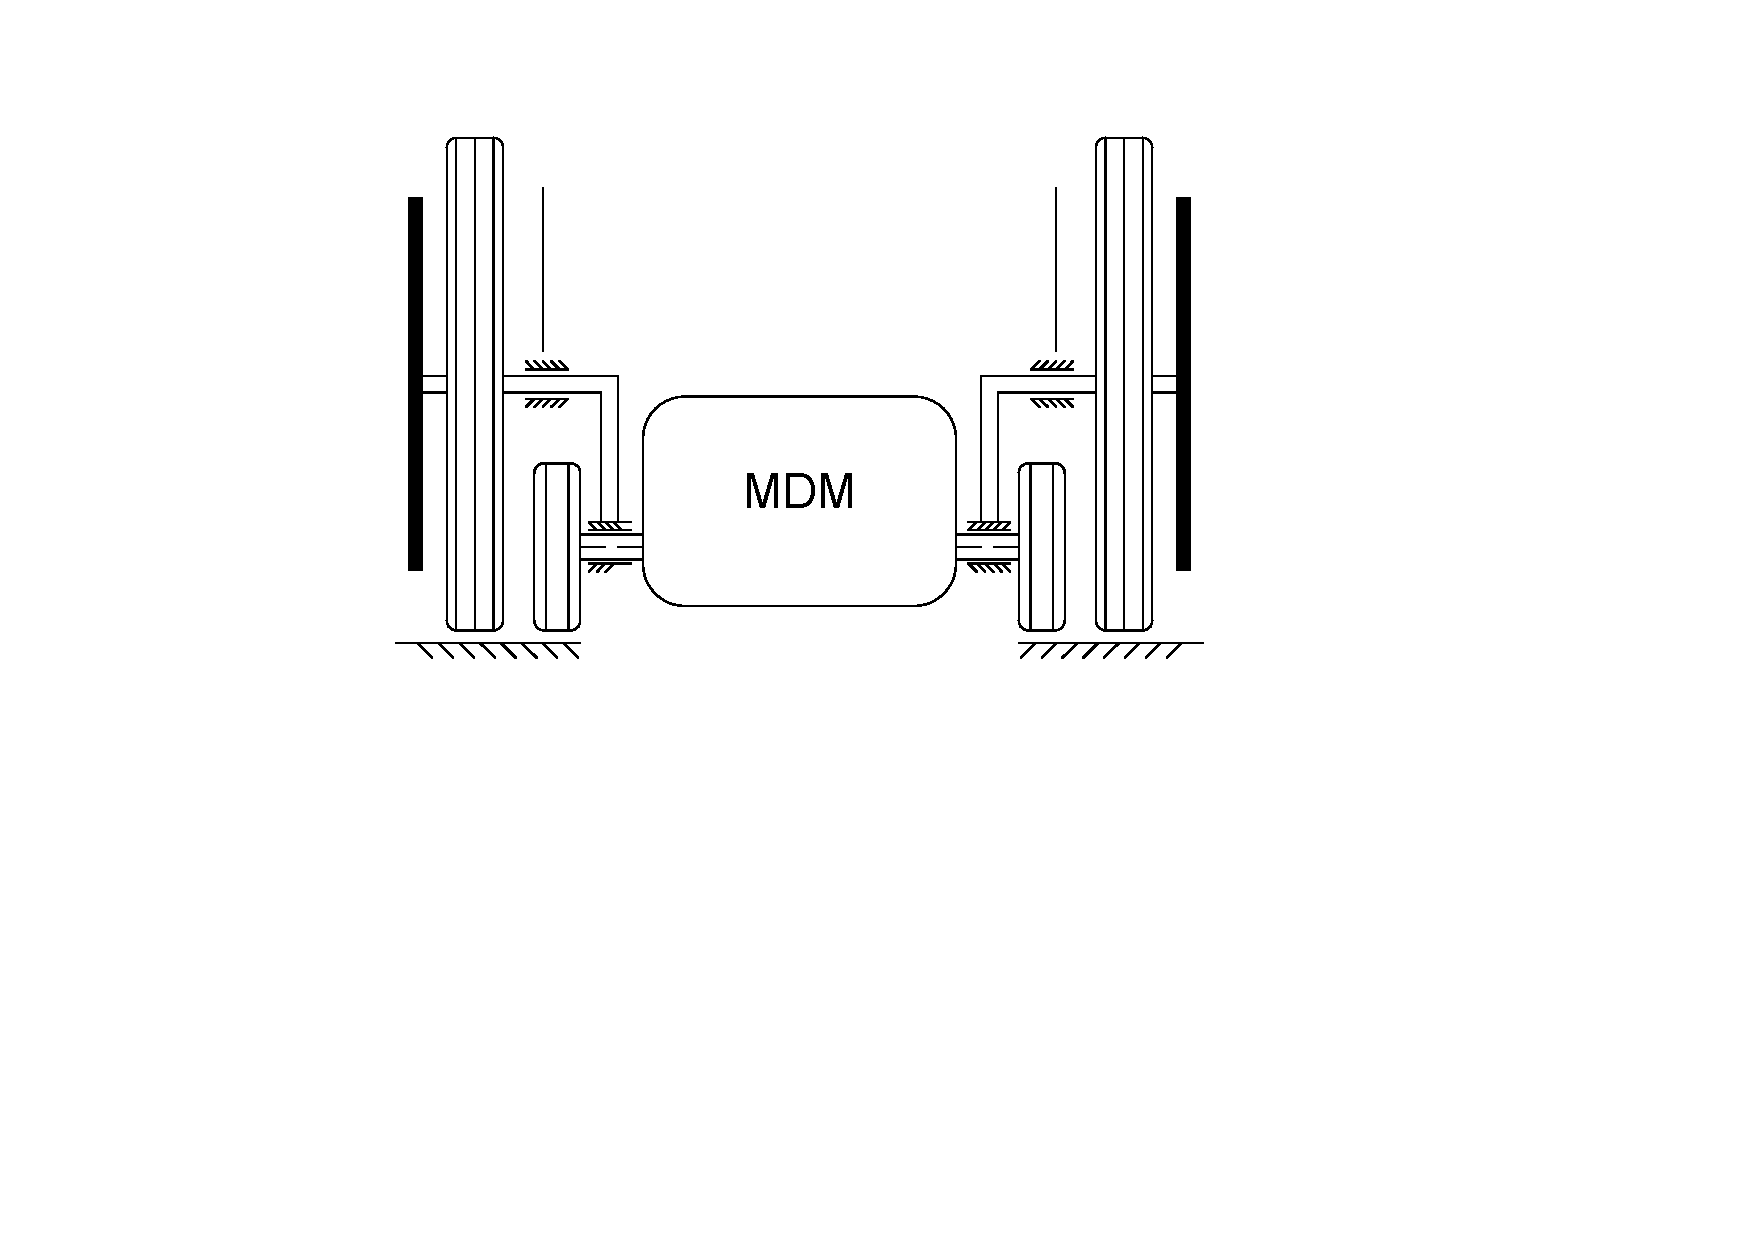
\includegraphics[width=0.6\textwidth]{fig/MDM_modified.pdf}
	\caption{机电驱动模块(MDM, \textit{mechatronic drive module})简图。}\label{fig:MDM_modified} % schematic diagram
\end{figure*}
%%%%%%%%%%%%%%%%%

为了研究有助于系统动态行为的不同组件,机电驱动模块与主体结构分离,基本布局如图~\ref{fig:MDM_modified} 所示。它包括使用速度减小的机械齿轮以及电动轮连接到系统的方式。轴上的旋转阻尼器和扭转弹簧的小值已经集中在一起并分别由 $R_s$ 和 $C_s$ 表示。

由此我们构建了相关的键图模型,它仅代表从电动推进轮椅中提取的机电一体化驱动模块系统如图~\ref{fig:MDM_scheme} 所示的动态特性的组件。

%%%%%%%%%%%%%%%%%
\begin{figure*}[!h]
	\centering
	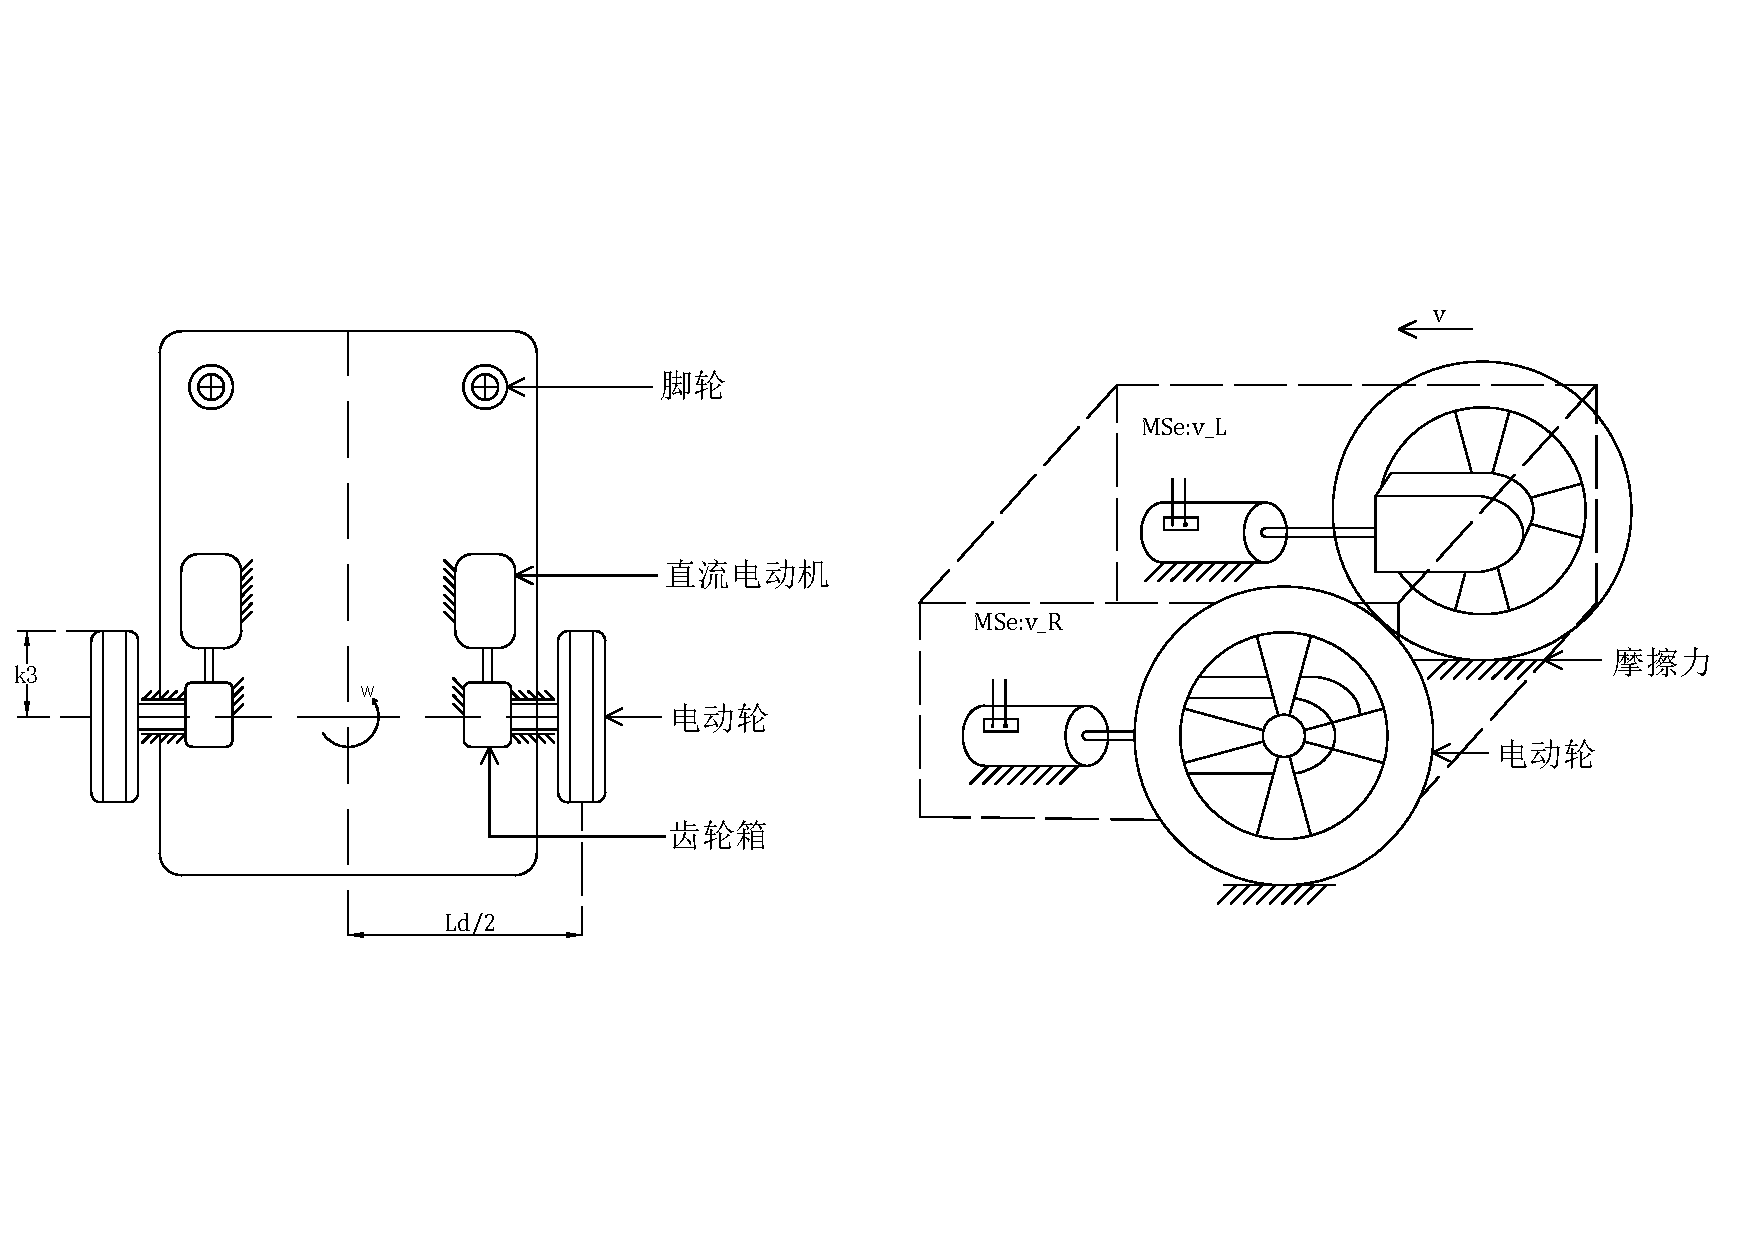
\includegraphics[width=1\textwidth]{fig/MDM_scheme.pdf}
	\caption{机电驱动模块主要结构示意。}\label{fig:MDM_scheme} % schematic diagram
\end{figure*}
%%%%%%%%%%%%%%%%%

\clearpage

\subsection{电驱动电机模块键合图}

首先对他励直流电机进行分析建模。作为机电驱动模块的核心,该部分我们既考虑了电路结构(包括主电路以及他励电路),也考虑了在输出扭矩时的机械损失。

我们用 MSe:L,$ I_e $,$ R_e $ 来分别表示输入控制电压,电机电感和内阻;用 $ J_r $,$ R_b $,$ C_s $,$ R_s $,$ k_1 $来分别表示转子转动惯量,电机轴承阻尼,电机输出转矩,电机输出轴阻尼和电机扭矩系数。如下图~\ref{fig:separately_excited_dc_motor}可见。根据电系统特点,我们标出相关共势点,为后续分析做准备。

%%%%%%%%%%%%%%%%%
\begin{figure*}[!h]
	\centering
	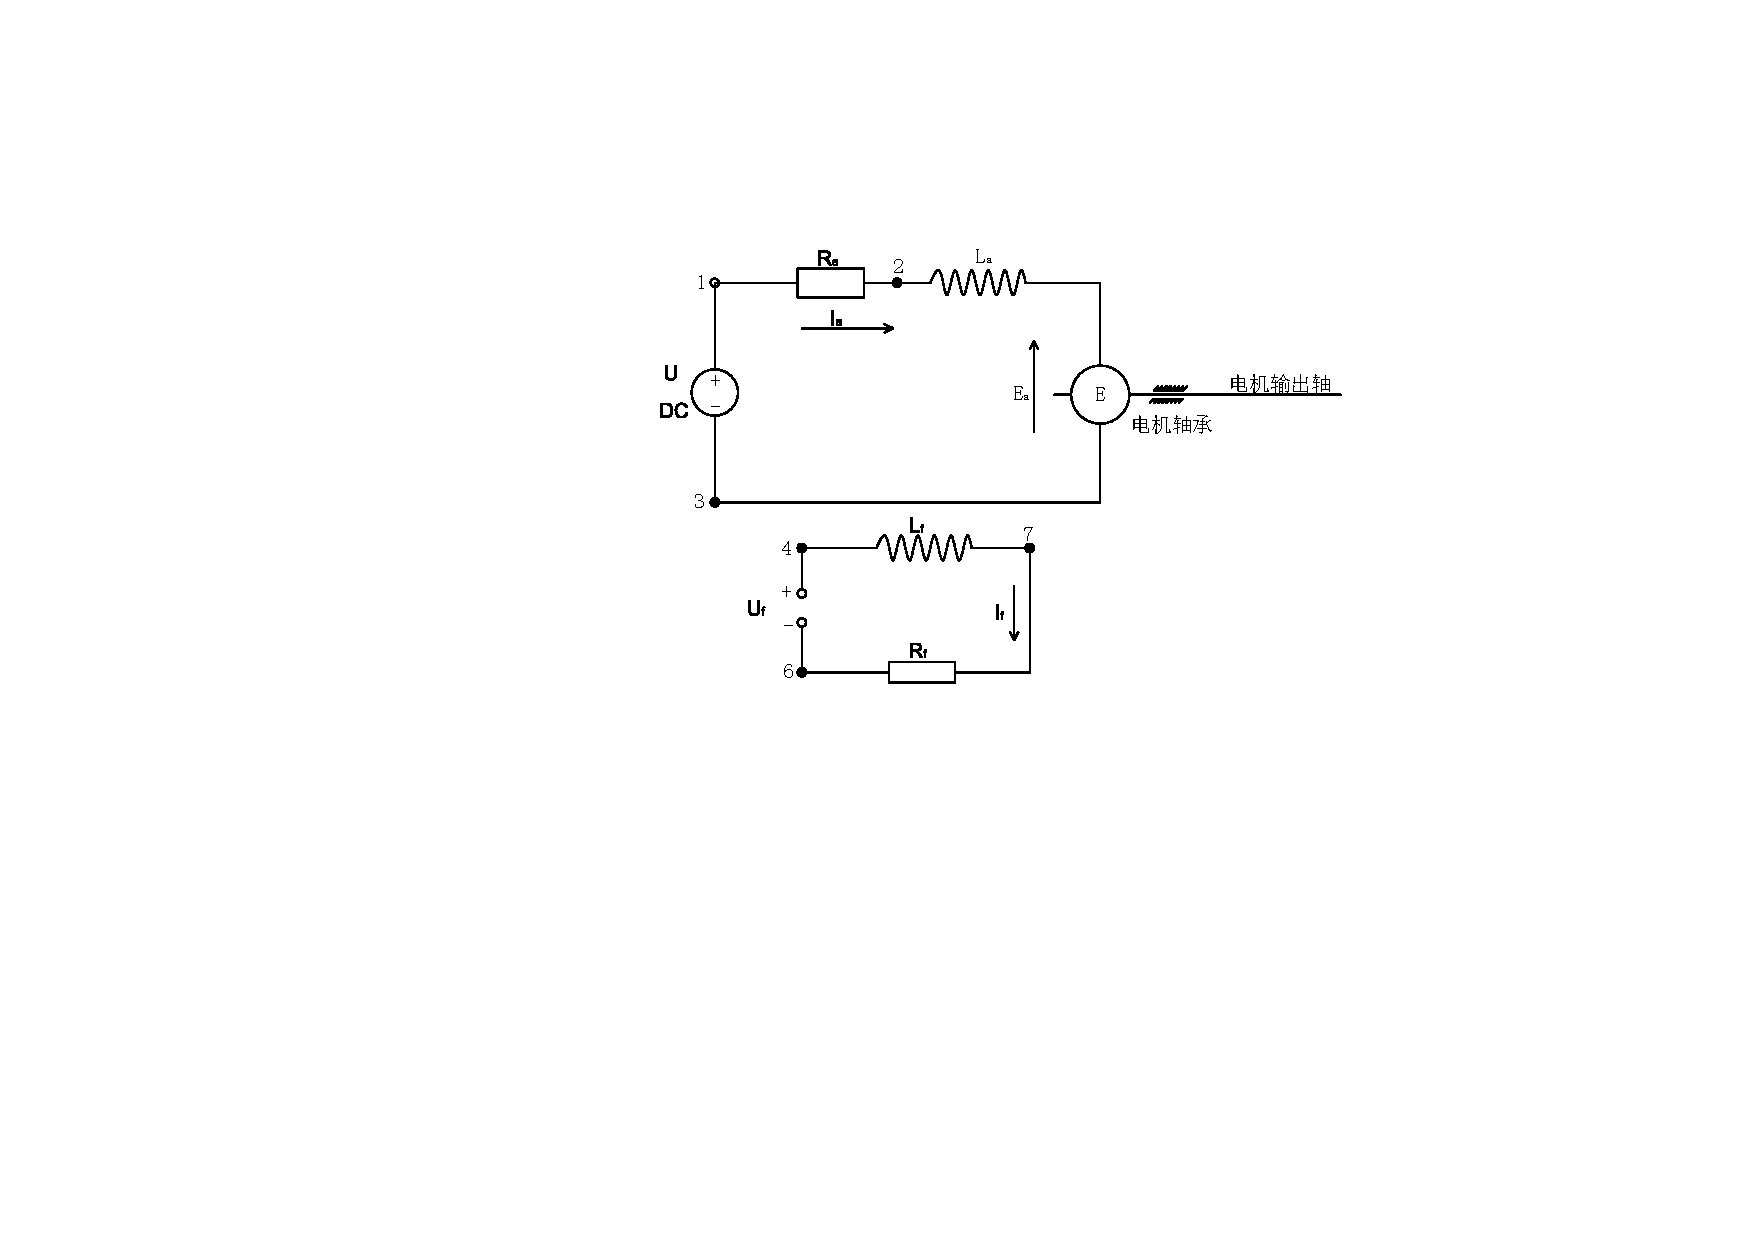
\includegraphics[width=1.05\textwidth]{fig/separately_excited_dc_motor.pdf}
	\caption{他励直流电机原理简图。}\label{fig:separately_excited_dc_motor} % schematic diagram
\end{figure*}
%%%%%%%%%%%%%%%%%

以下为具体建模过程:

\begin{enumerate}
	\item 定义电流的正方向以及电机输出轴的转速正方向如图~\ref{fig:separately_excited_dc_motor} 所示。
	
	\item 电路主回路和励磁回路分别有3个共势点,电机轴包括2个速度结点。
	如下图所示:
	%%%%%%%%%%%%%%%%%
	\begin{figure*}[!h]
		\centering
		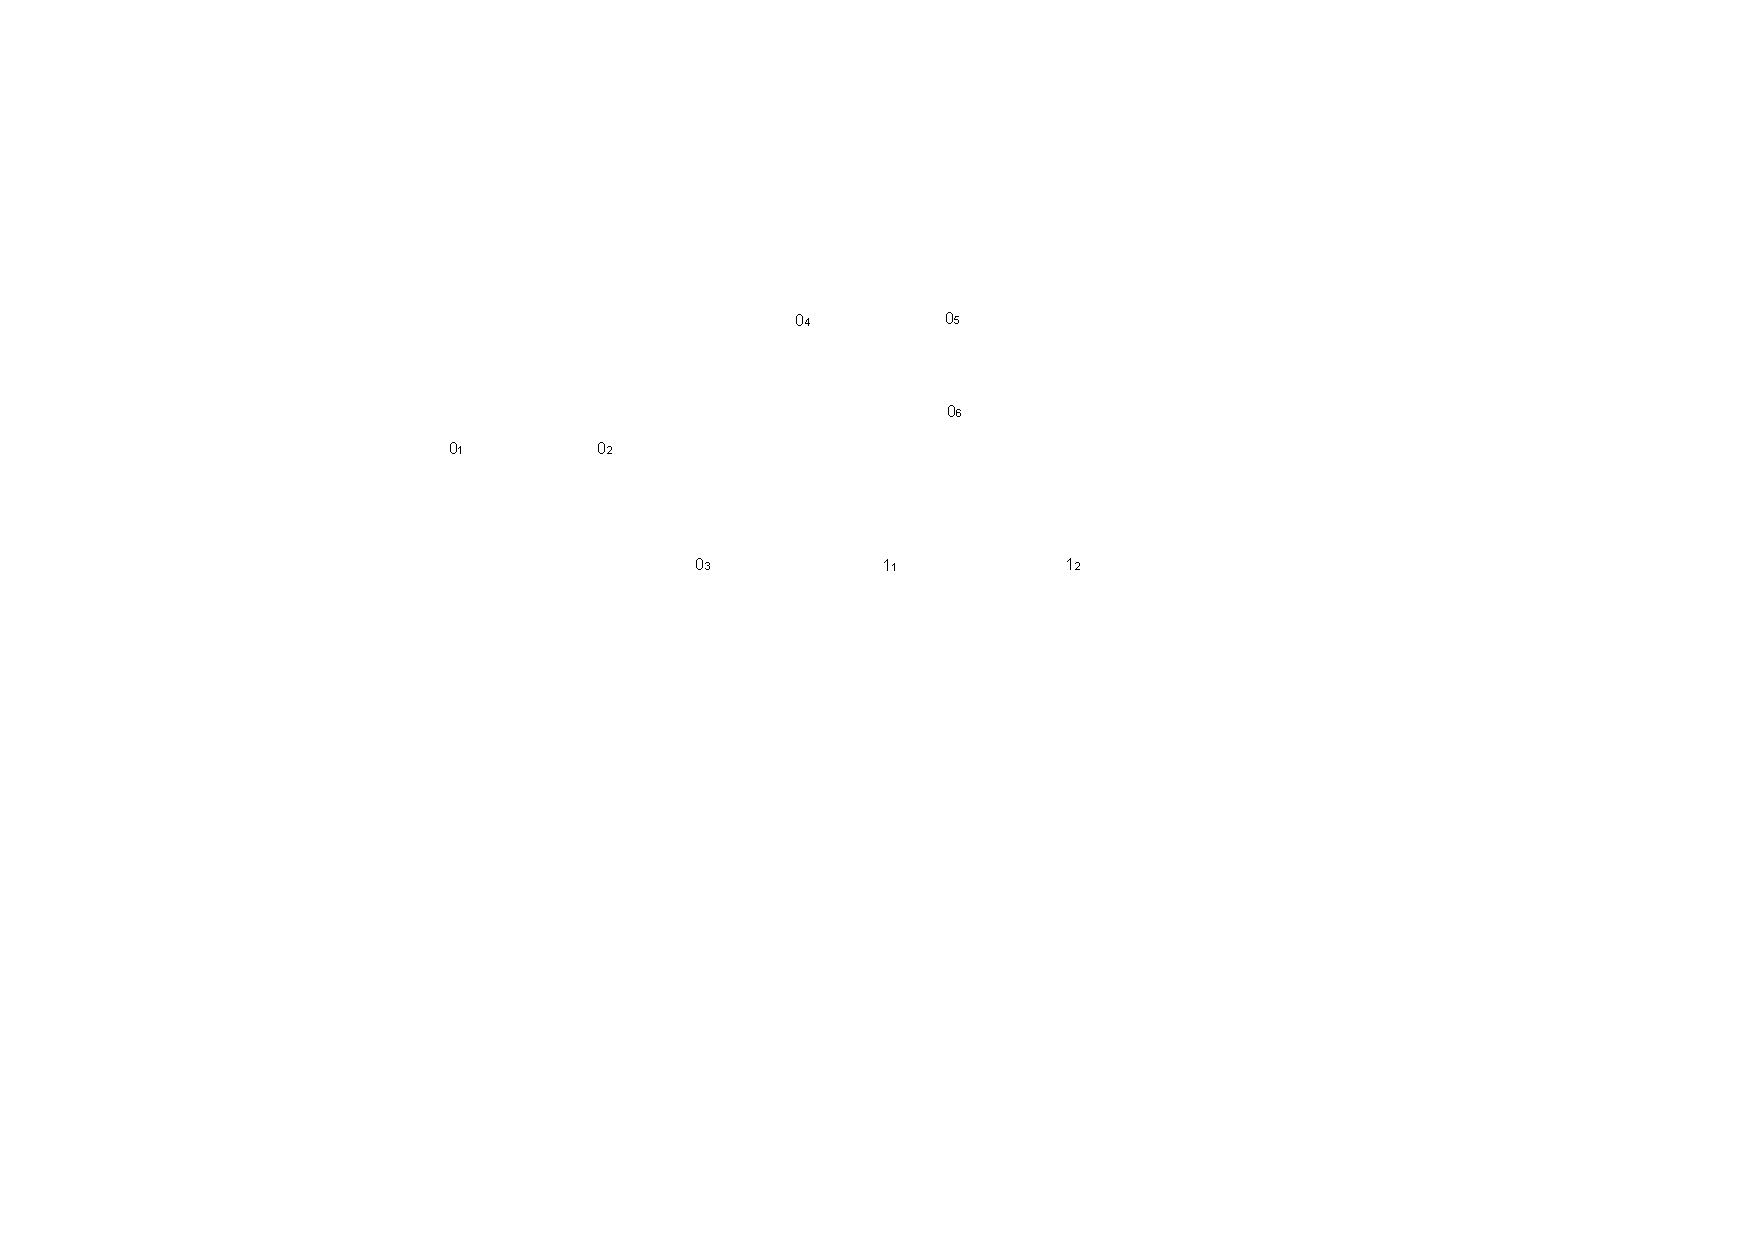
\includegraphics[width=1.05\textwidth]{fig/4_1_bond.pdf}
		\caption{电驱动模块电机模型键合图——标注0-结与1-结。}\label{fig:4_1_bond}
	\end{figure*}
	%%%%%%%%%%%%%%%%%
	
	\clearpage
	
	\item 添加源和RCI元件。同时根据功率方向画出半箭头。
	如下图所示:
	%%%%%%%%%%%%%%%%%
	\begin{figure*}[!h]
		\centering
		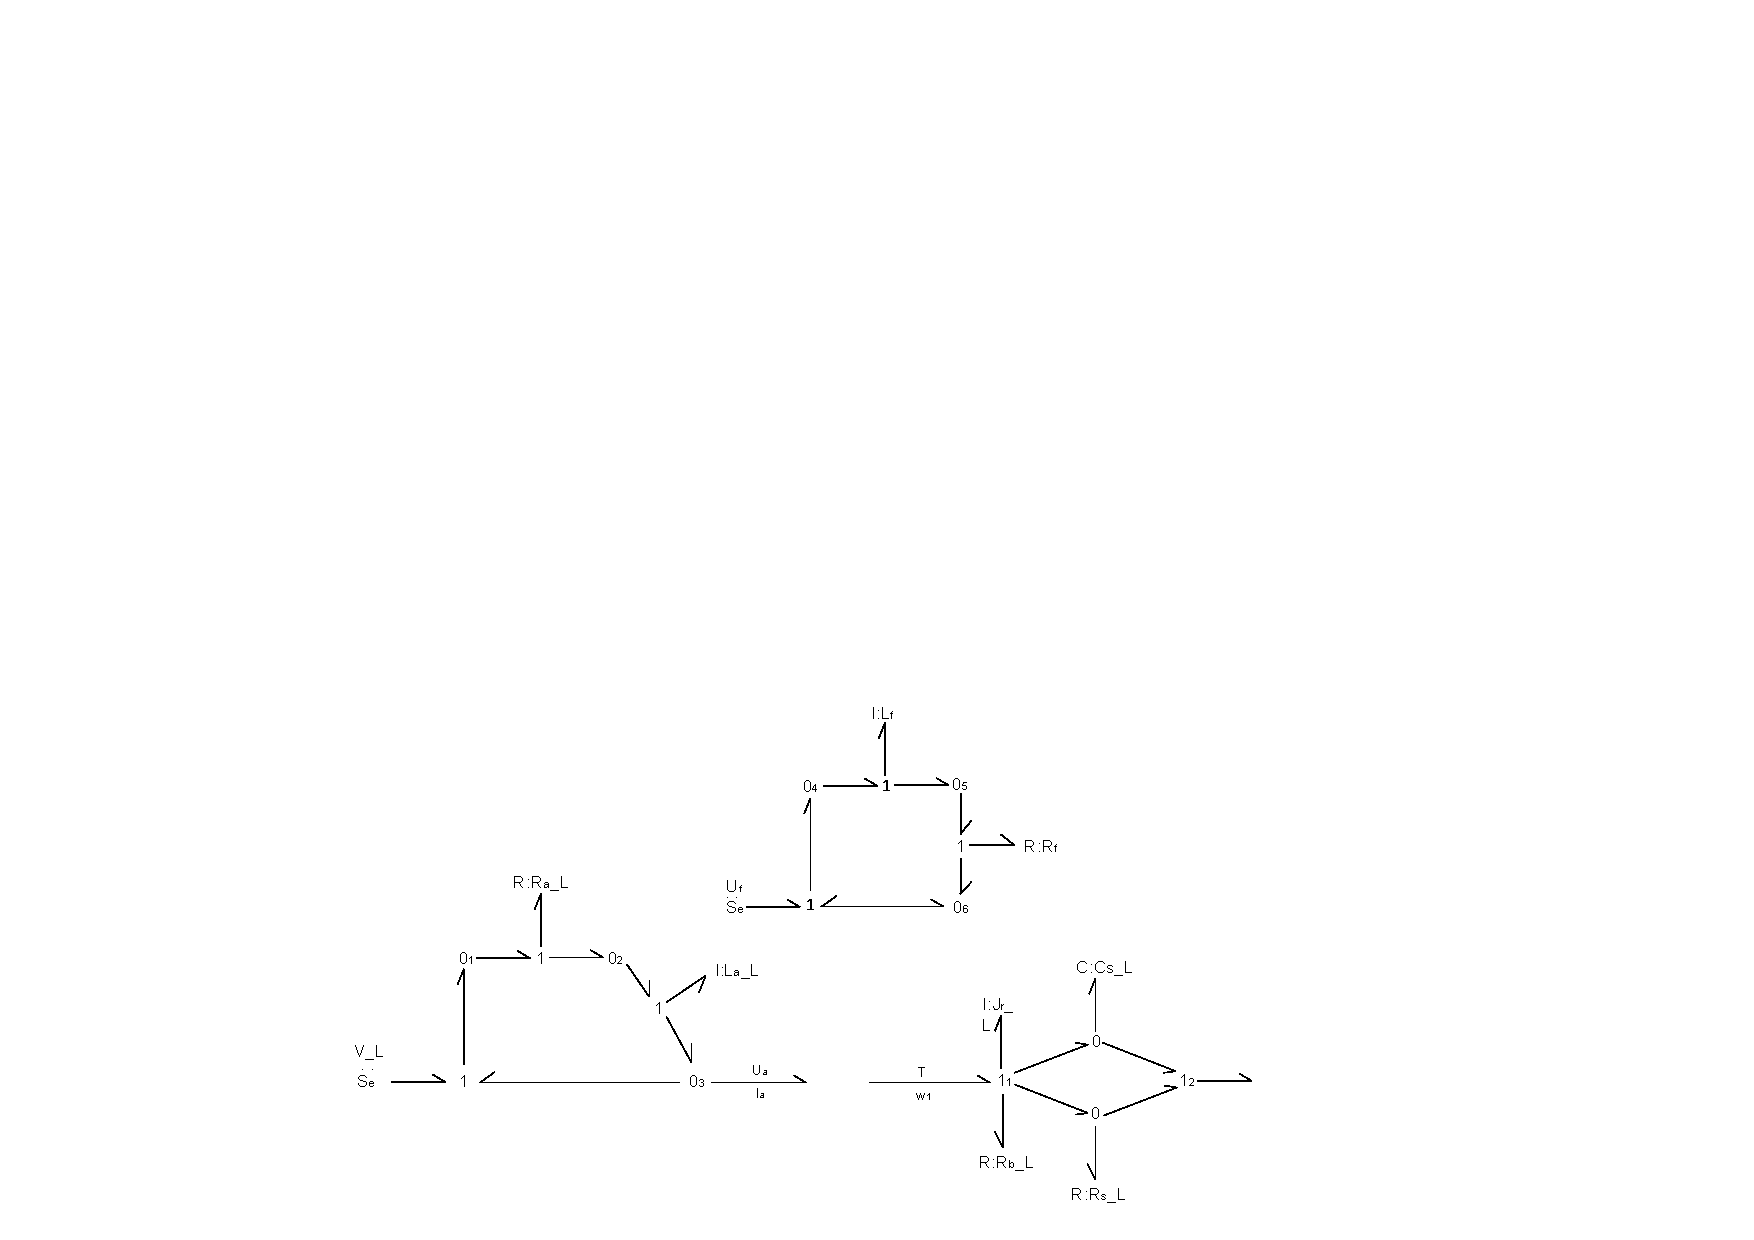
\includegraphics[width=0.92\textwidth]{fig/4_2_bond.pdf}
		\caption{电驱动模块电机模型键合图——添加源和RCI元件。}\label{fig:4_2_bond}
	\end{figure*}
	%%%%%%%%%%%%%%%%%
	
	\item 在电系统和机械系统之间添加回转器。根据对应数学关系:
	%%%%%%%%%%%%%%%%%%%%%%%%%%
	\begin{equation}
	\label{equ:U_a}
	U_a
	=
	\left( C_e \Phi_e \frac{60}{2 \pi}\right) * w_1
	\ ,
	\end{equation}
	%%%%%%%%%%%%%%%%%%%%%%%%%%
	%%%%%%%%%%%%%%%%%%%%%%%%%%
	\begin{equation}
	\label{equ:T}
	T
	=\
	(C_t \Phi_e) * I_a
	\ .
	\end{equation}
	%%%%%%%%%%%%%%%%%%%%%%%%%%
	
	同时根据功率方向画出半箭头。
	如下图所示:	
	%%%%%%%%%%%%%%%%%
	\begin{figure*}[!h]
		\centering
		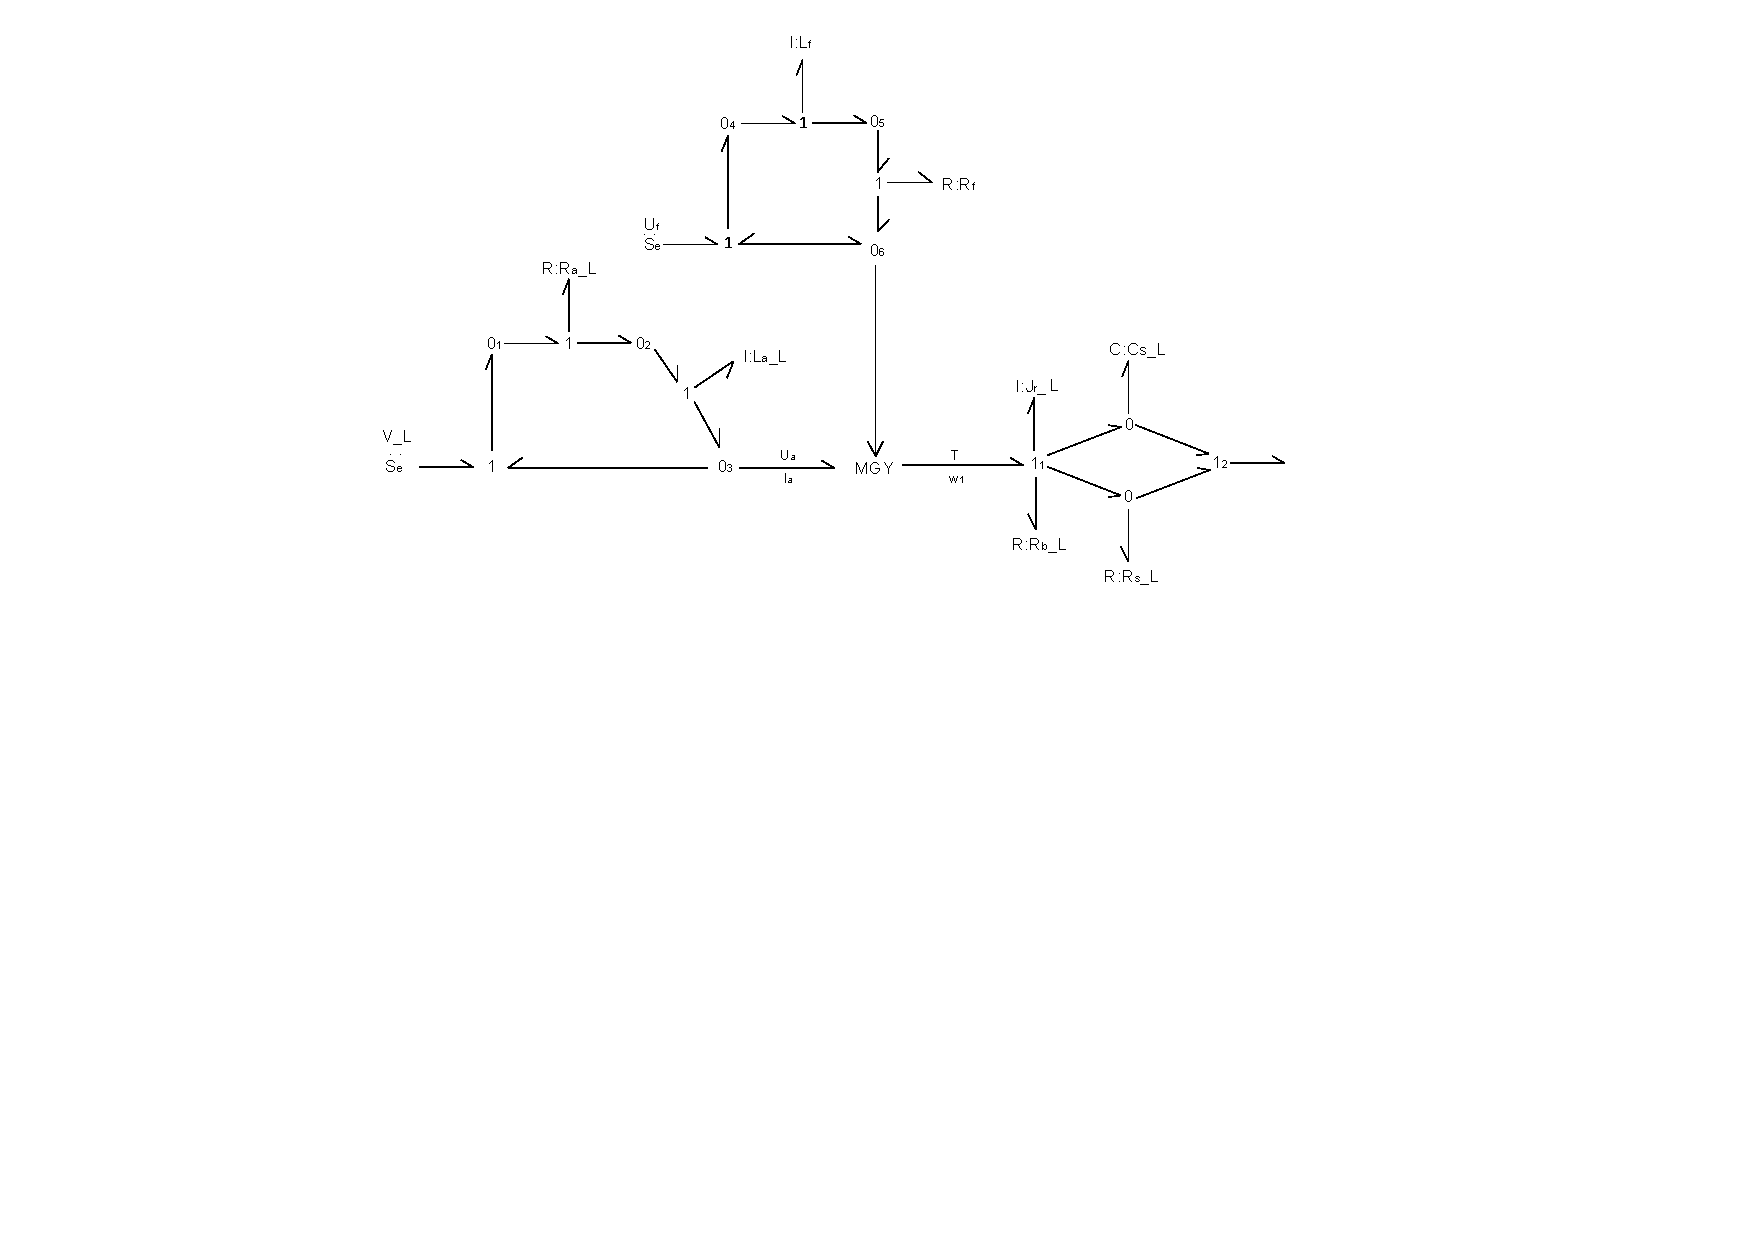
\includegraphics[width=0.92\textwidth]{fig/4_3_bond.pdf}
		\caption{电驱动模块电机模型键合图——添加回转器。}\label{fig:4_3_bond}
	\end{figure*}
	%%%%%%%%%%%%%%%%%
	
	\item 电机模型电系统部分化简。根据电路图可知,03和06接地,因此可以对上面键合图进行化简。
	如下图所示:
	%%%%%%%%%%%%%%%%%
	\begin{figure*}[!h]
		\centering
		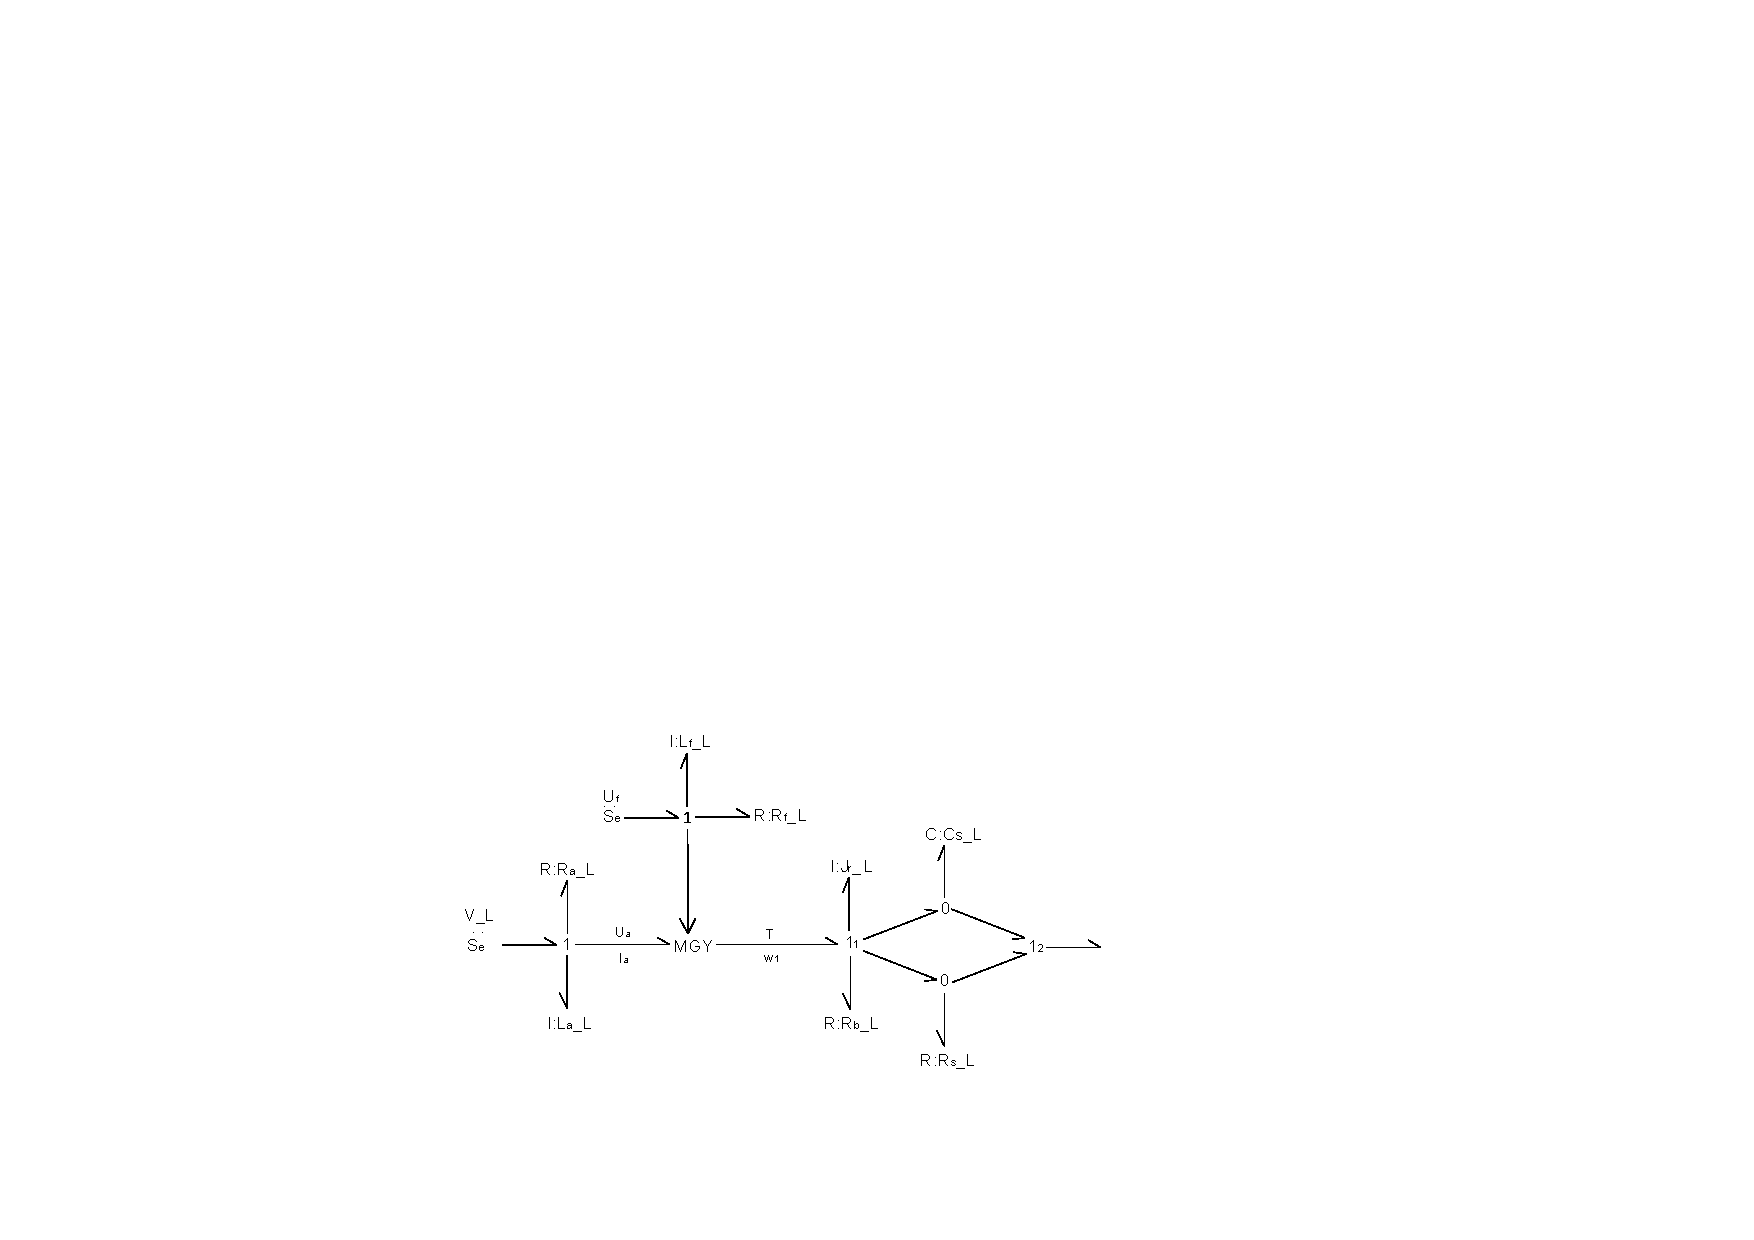
\includegraphics[width=1.2\textwidth]{fig/4_4_bond.pdf}
		\caption{电机模型电系统键合图部分化简。}\label{fig:4_4_bond}
	\end{figure*}
	%%%%%%%%%%%%%%%%%
	
	\item 电机模型功率环化简。
	如下图所示:
	%%%%%%%%%%%%%%%%%
	\begin{figure*}[!h]
		\centering
		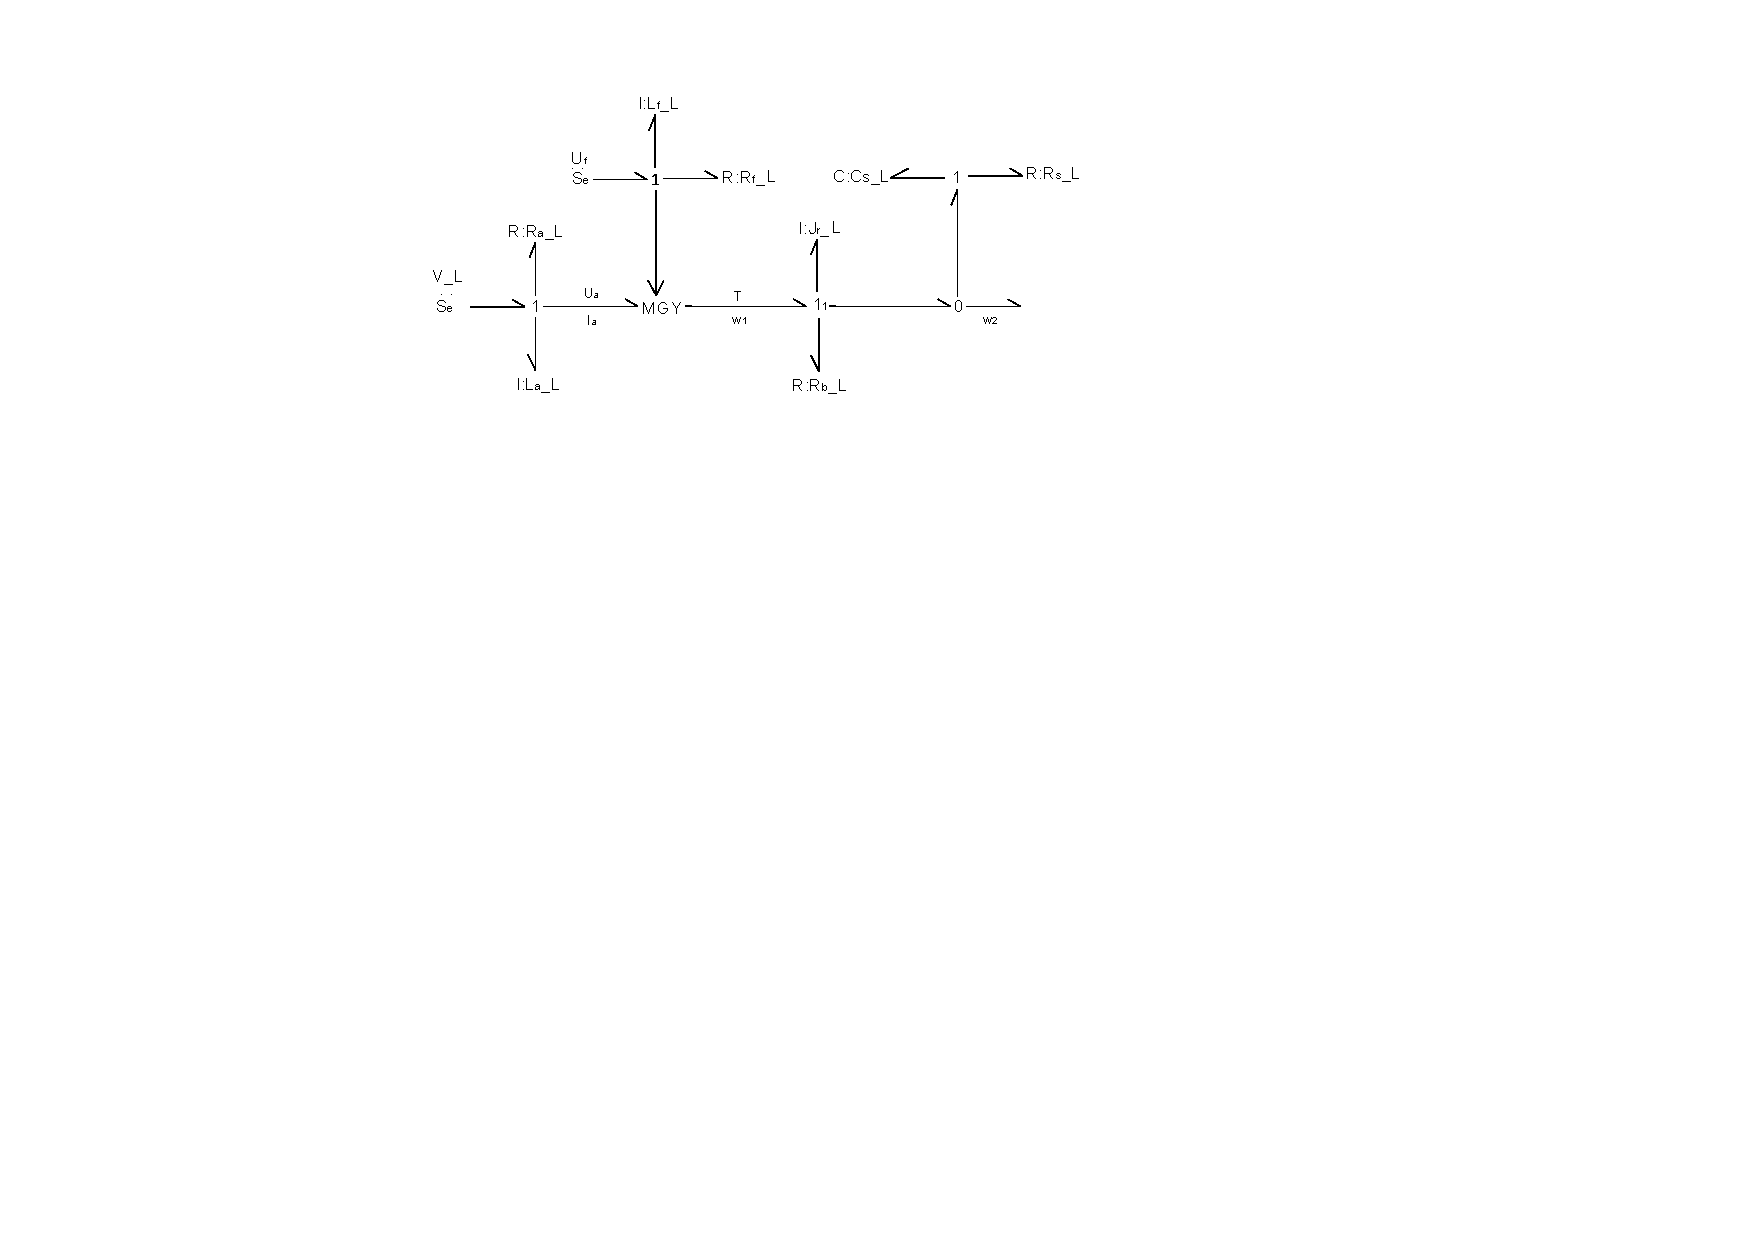
\includegraphics[width=1\textwidth]{fig/4_5_bond.pdf}
		\caption{电机模型键合图功率环化简。}\label{fig:4_5_bond}
	\end{figure*}
	%%%%%%%%%%%%%%%%%
	
\end{enumerate}

\clearpage

\subsection{电驱动模块其余部分键合图}

以下为具体建模过程:

\begin{enumerate}
	\item 对于每一个确定的速度,标注速度1-结。
	本装置一共有 6 个确定的(角)速度,即左/右后轮角速度,左/右后轮线速度,电驱动模块质心速度和电驱动模块质心角速度。
	如下图所示:
	%%%%%%%%%%%%%%%%%
	\begin{figure*}[!h]
		\centering
		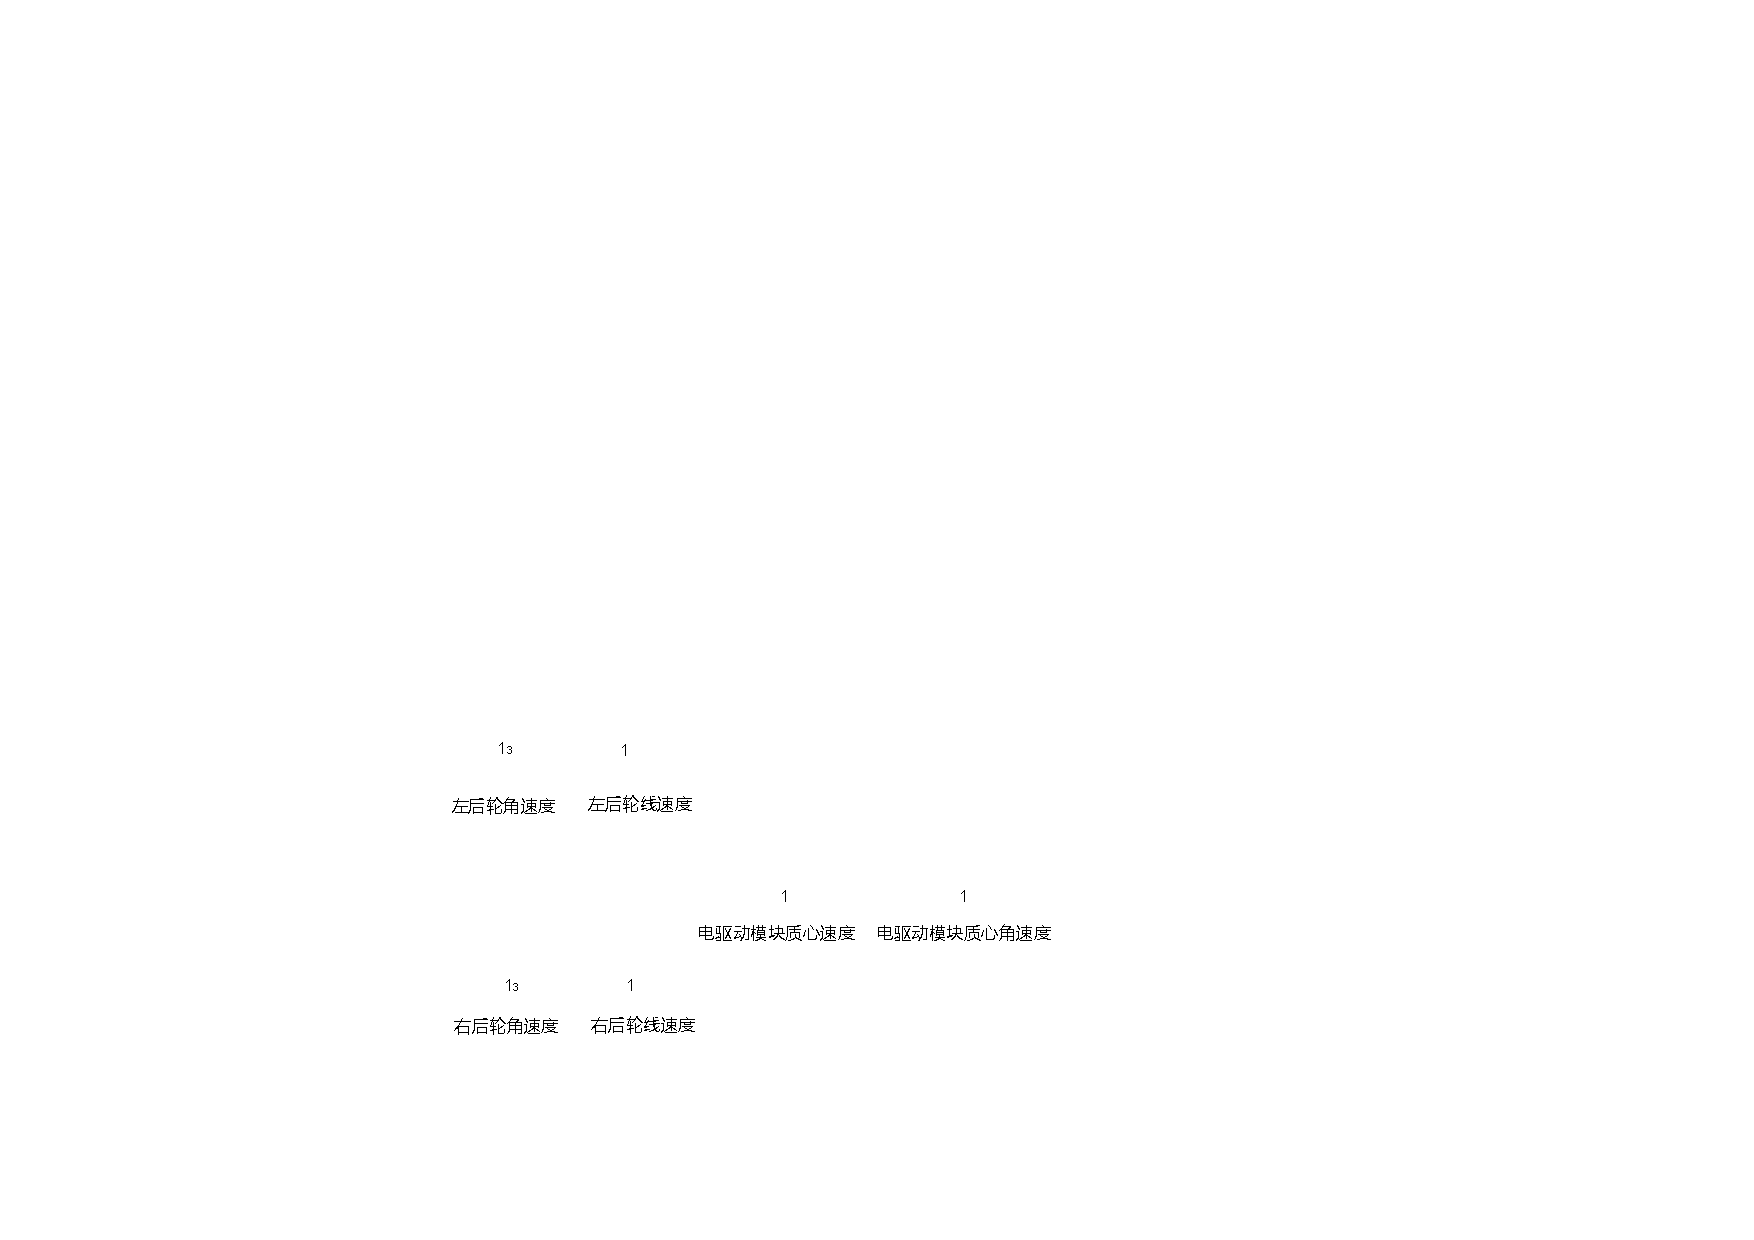
\includegraphics[width=0.7\textwidth]{fig/4_6_bond.pdf}
		\caption{电驱动模块其余部分键合图——标注速度1-结。}\label{fig:4_6_bond}
	\end{figure*}
	%%%%%%%%%%%%%%%%%
	
	\item 添加RCI元件。同时根据功率方向画出半箭头。
	如下图所示:
	%%%%%%%%%%%%%%%%%
	\begin{figure*}[!h]
		\centering
		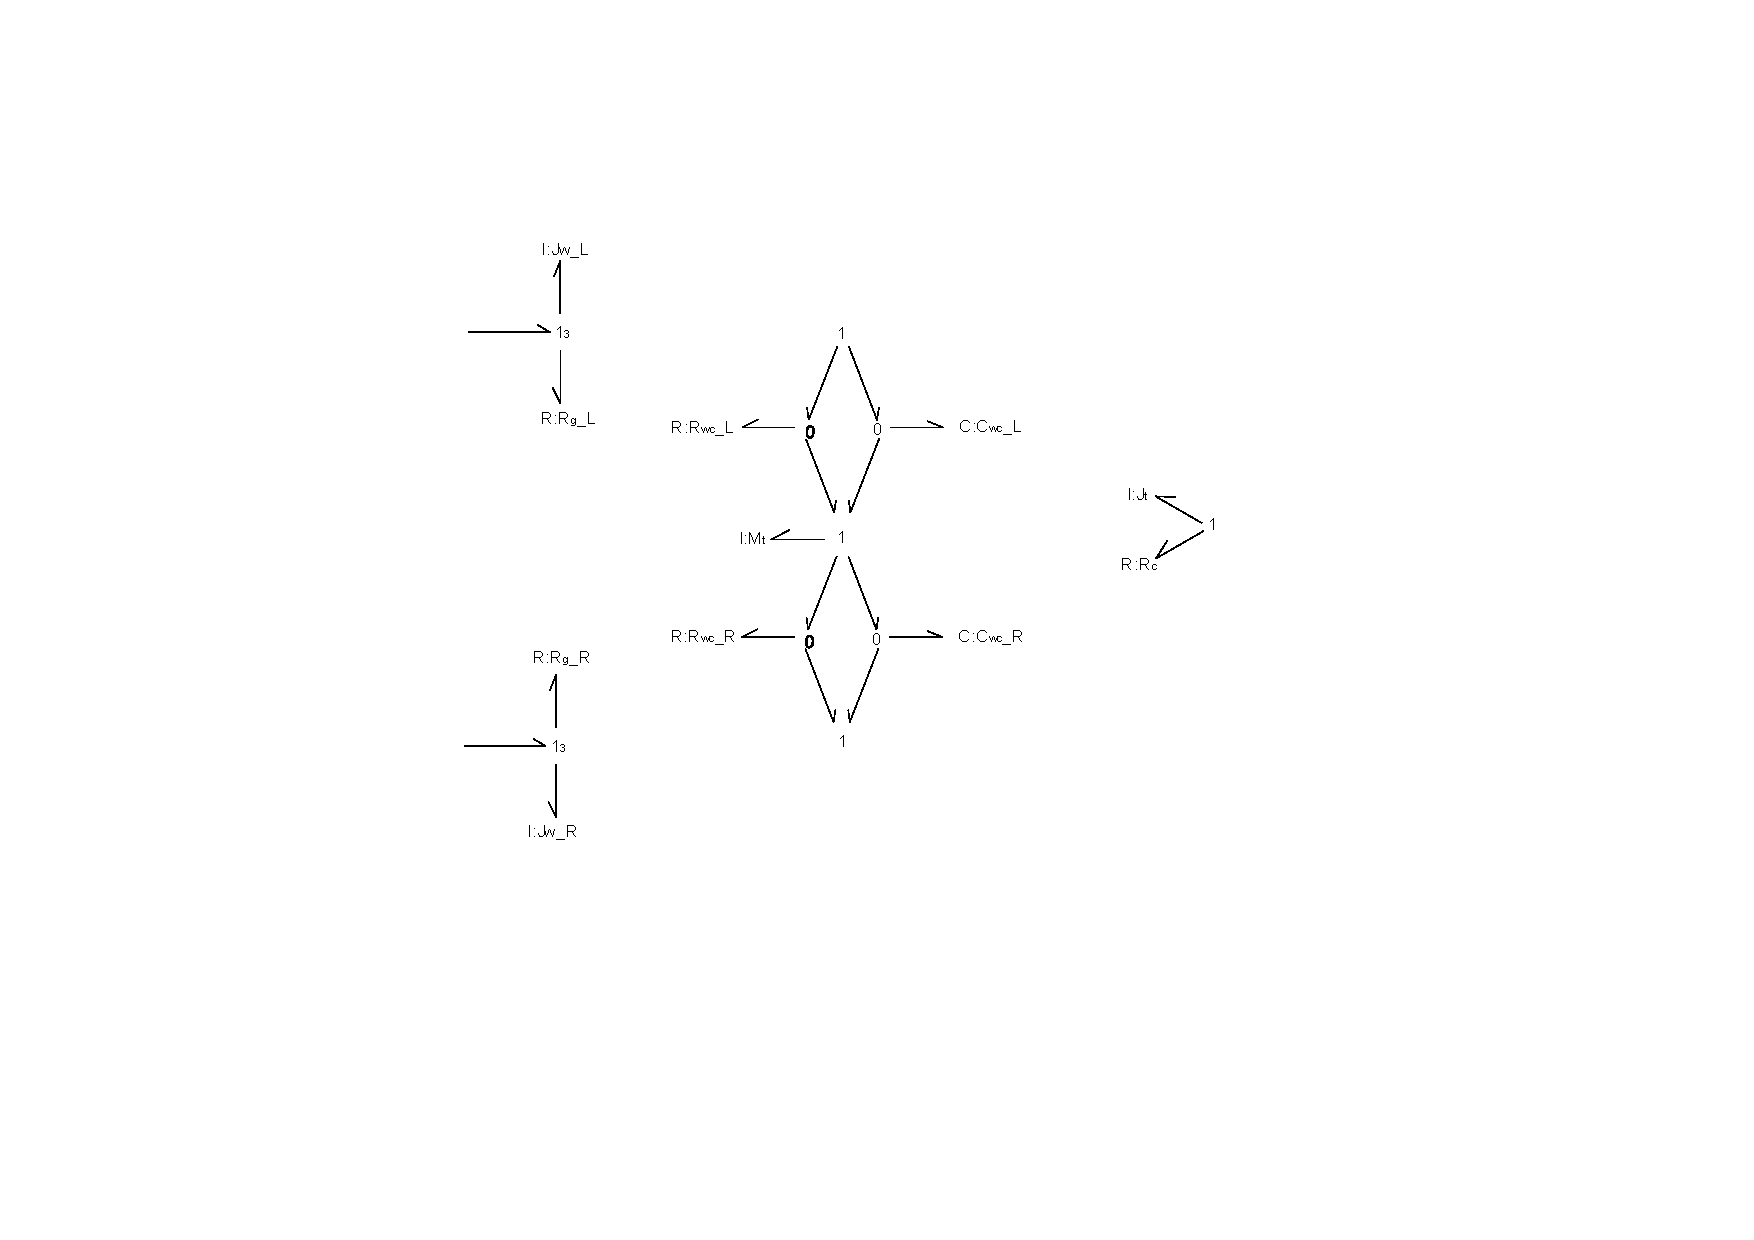
\includegraphics[width=0.85\textwidth]{fig/4_7_bond.pdf}
		\caption{电驱动模块其余部分键合图——添加RCI元件。}\label{fig:4_7_bond}
	\end{figure*}
	%%%%%%%%%%%%%%%%%
	
	\item 添加变换器。其中,电驱动模块左右后轮的线速度和整个的质心角速度之间存在下面的关系,所以所添加的变换器为可调变换器。
	%%%%%%%%%%%%%%%%%%%%%%%%%%
	\begin{equation}
	\label{equ:V_L}
	V_L
	=
	V_{CG}-W_{CG} \times \frac{L_d}{2} \times \cos \theta
	\ ,
	\end{equation}
	%%%%%%%%%%%%%%%%%%%%%%%%%%
	%%%%%%%%%%%%%%%%%%%%%%%%%%
	\begin{equation}
	\label{equ:V_R}
	V_R
	=
	V_{CG}+W_{CG} \times \frac{L_d}{2} \times \cos \theta
	\ ,
	\end{equation}
	%%%%%%%%%%%%%%%%%%%%%%%%%%
	
	同时根据功率方向画出半箭头。	
	如下图所示:
	%%%%%%%%%%%%%%%%%
	\begin{figure*}[!h]
		\centering
		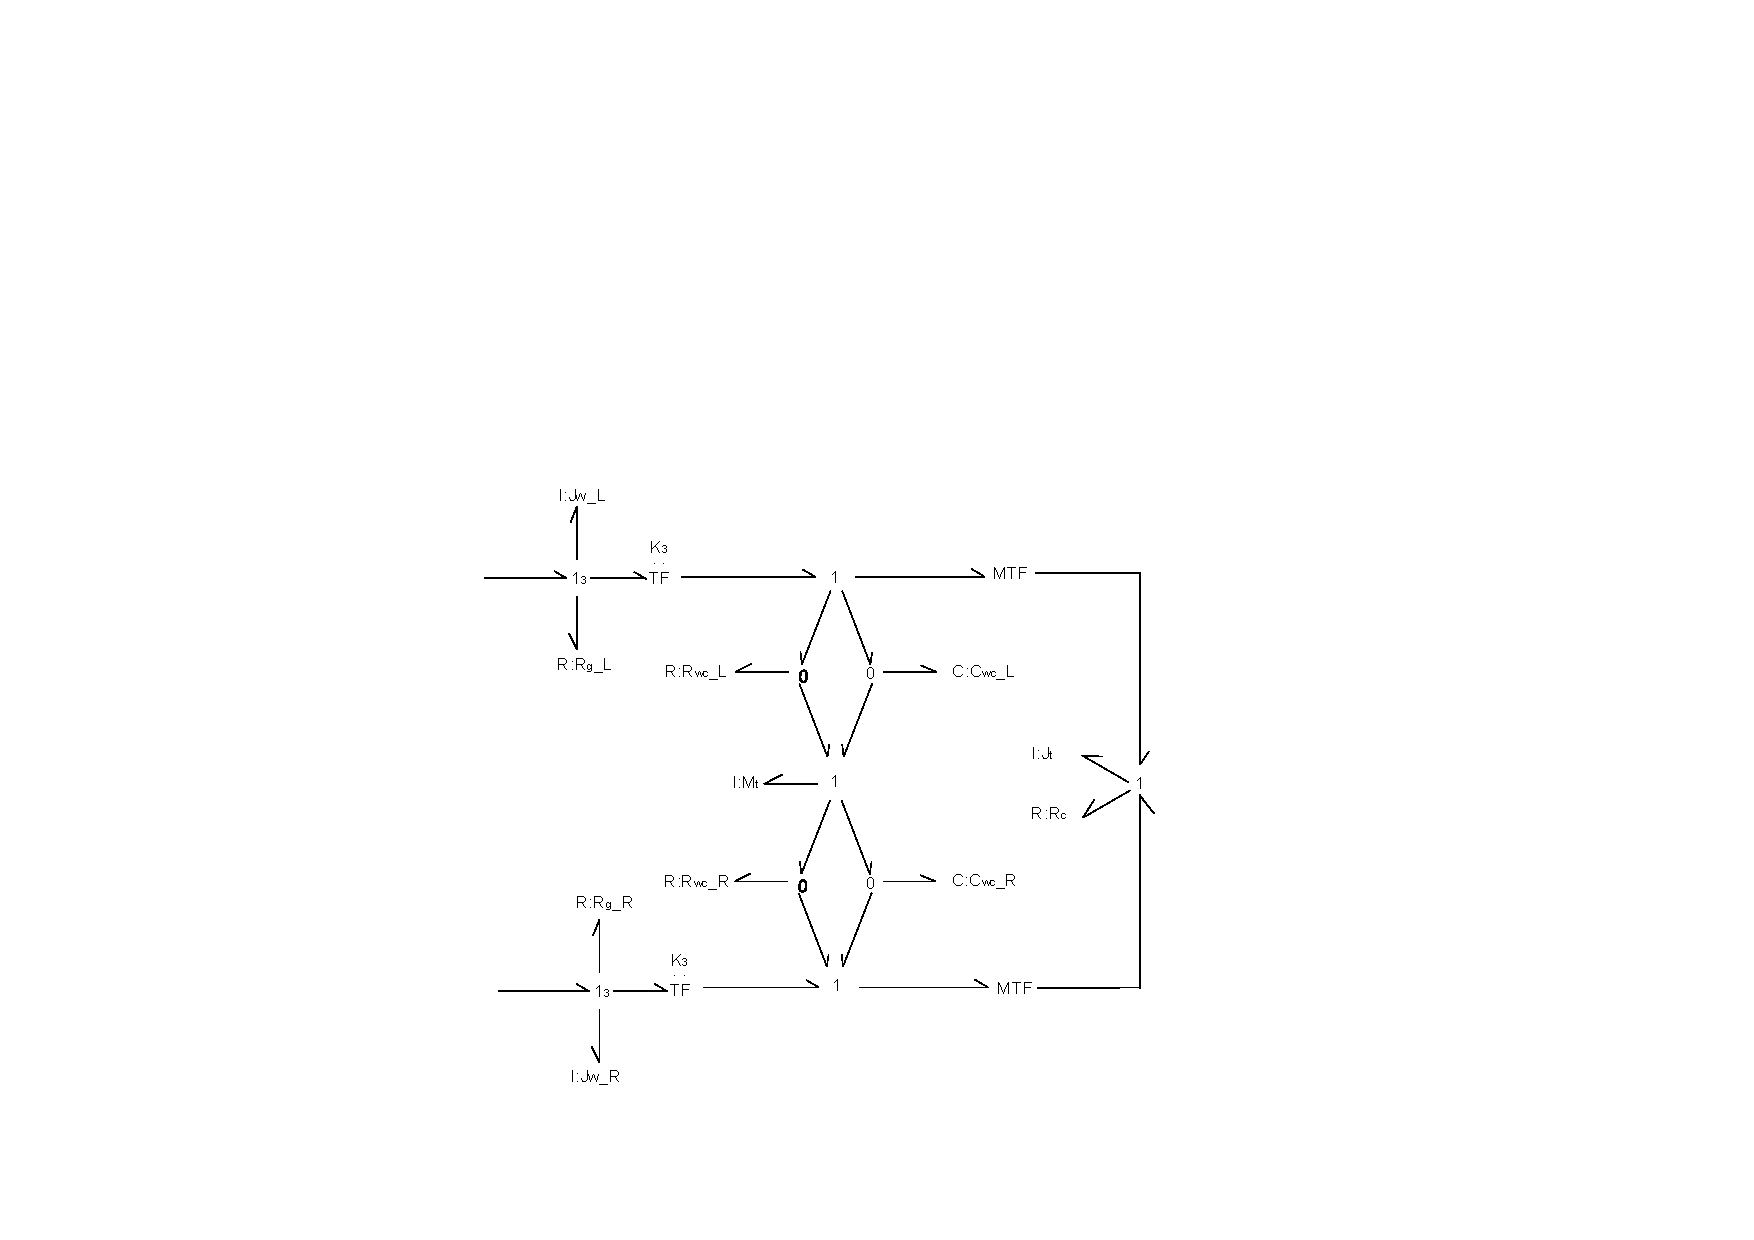
\includegraphics[width=0.85\textwidth]{fig/4_8_bond.pdf}
		\caption{电驱动模块其余部分键合图——添加变换器。}\label{fig:4_8_bond}
	\end{figure*}
	%%%%%%%%%%%%%%%%%
	
	\clearpage
	
	\item 模型功率环化简。
	如下图所示:
	%%%%%%%%%%%%%%%%%
	\begin{figure*}[!h]
		\centering
		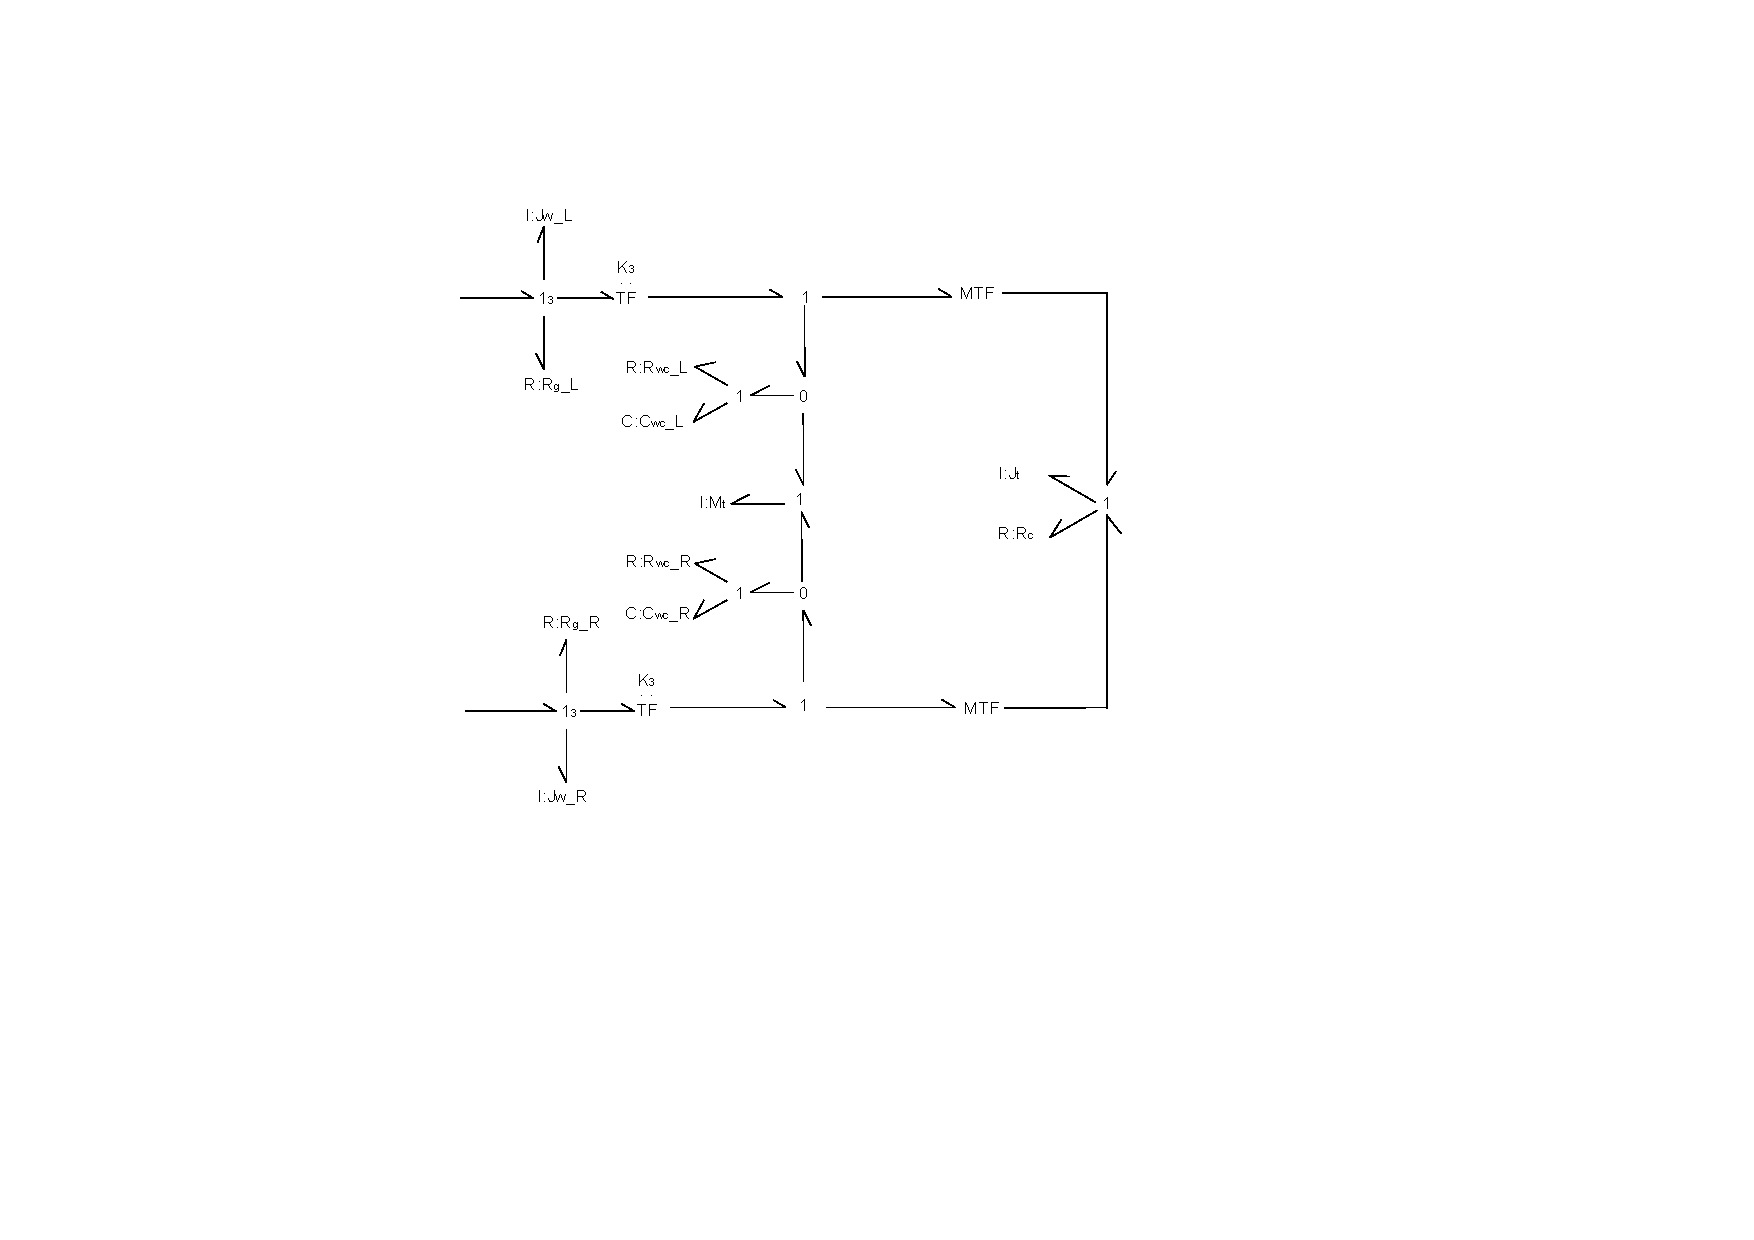
\includegraphics[width=0.85\textwidth]{fig/4_9_bond.pdf}
		\caption{电驱动模块其余部分键合图功率环化简。}\label{fig:4_9_bond}
	\end{figure*}
	%%%%%%%%%%%%%%%%%
	
\end{enumerate}

\subsection{机电驱动模块键合图}

相比于图~\ref{fig:4_5_bond} 和图~\ref{fig:4_9_bond} ,他励直流电动机与电动小车机械部分结合,它们之间通过一个减速齿轮箱连接,所以键合图连接的地方需要添加一个变换器,得到图~\ref{fig:4_10_bond}(见下页)。

%%%%%%%%%%%%%%%%%
\begin{figure*}[!t]
	\centering
	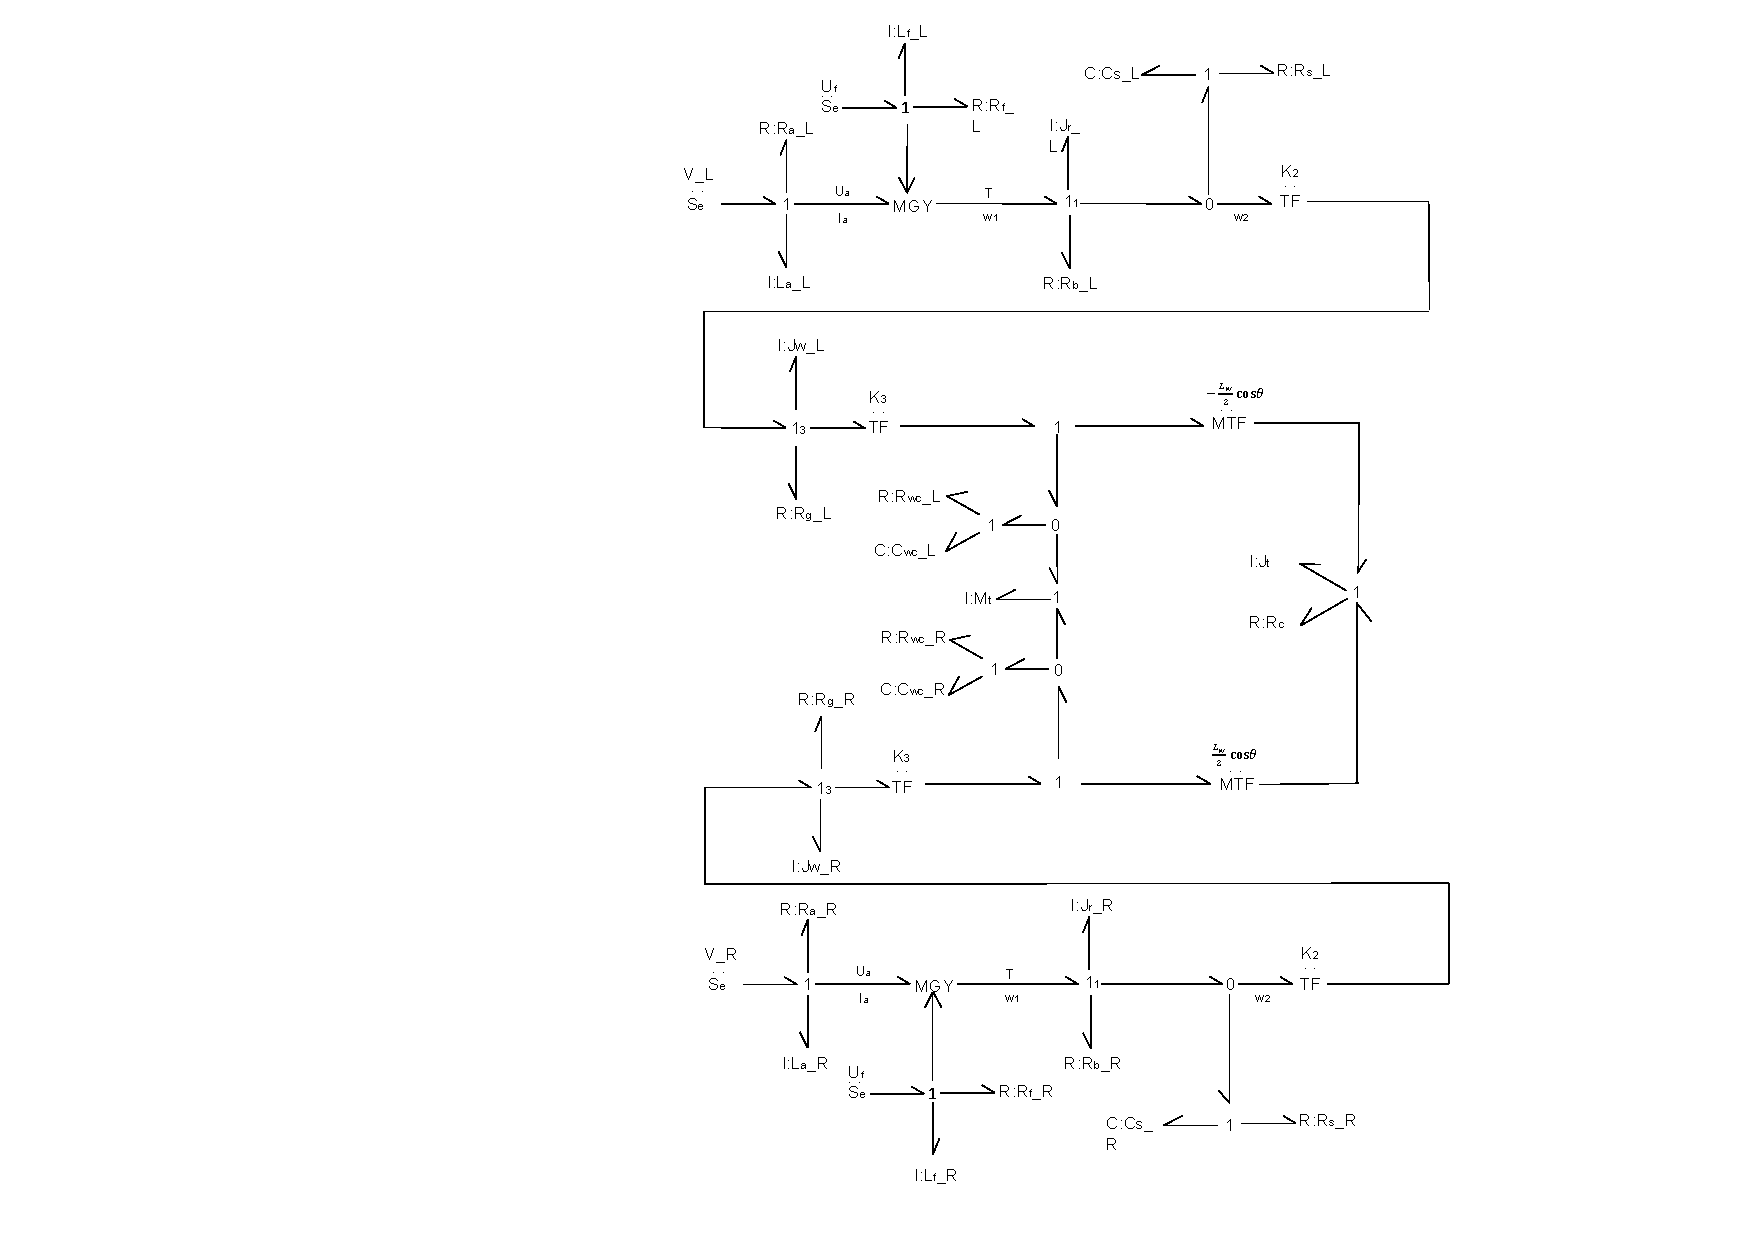
\includegraphics[width=0.96\textwidth]{fig/4_10_bond.pdf}
	\caption{机电驱动模块键合图——两部分键合图拼接。}\label{fig:4_10_bond}
\end{figure*}
%%%%%%%%%%%%%%%%%

\clearpage

添加因果关系后,最终得到构成机电驱动模块的各个部件组件的键合图,如图~\ref{fig:part2_bond} 示。

%%%%%%%%%%%%%%%%%
\begin{figure*}[!h]
	\centering
	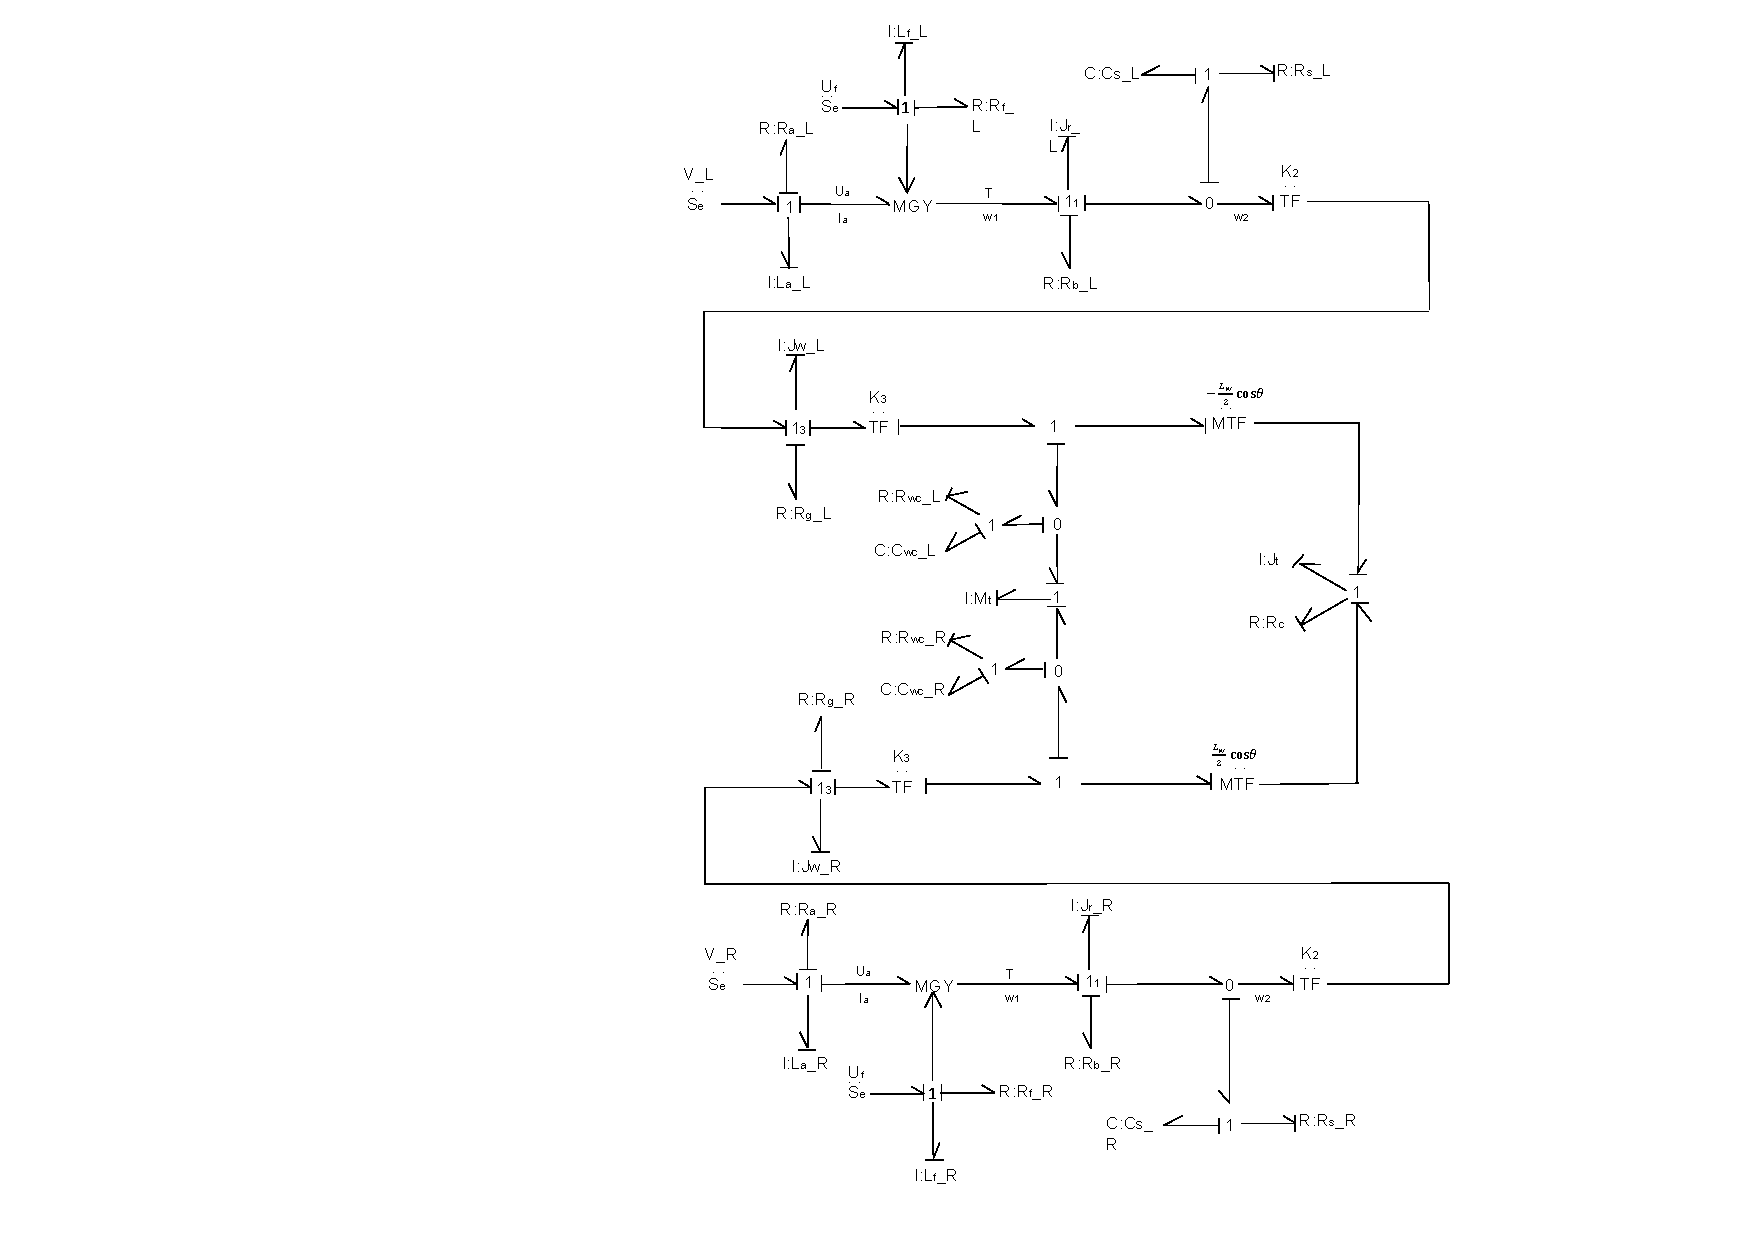
\includegraphics[width=0.92\textwidth]{fig/part2_bond.pdf}
	\caption{机电驱动模块键合图——总体键合图。}\label{fig:part2_bond}
\end{figure*}
%%%%%%%%%%%%%%%%%
